\documentclass[onecolumn]{article}
\usepackage[utf8]{inputenc}
\usepackage{cite}
\usepackage{geometry}
\usepackage{graphicx}
\usepackage{subfigure}
\usepackage[table,xcdraw]{xcolor}
\usepackage{amsmath}
\usepackage{float}
\geometry{left=2cm,right=2cm,top=2cm,bottom=4cm}

\usepackage{enumitem}
\setenumerate[1]{itemsep=0pt,partopsep=0pt,parsep=\parskip,topsep=5pt}
\setitemize[1]{itemsep=0pt,partopsep=0pt,parsep=\parskip,topsep=5pt}
\setdescription{itemsep=0pt,partopsep=0pt,parsep=\parskip,topsep=5pt}




\title{MTH 9899 Final Project Report}
\author{Group Name: Lexington Alpha\\
        Group Member: Yigao (Hugo) Liu, Haocheng (Frank) Gu,\\
        Chenyu (Phillip) Zhao, Zichao (David) Wang}
\date{May 22, 2019}

\begin{document}

\maketitle

\section{Trim Data}
\subsection{Observations before Trimming}
Before applying any trimming technique, we first have several observations:
\begin{itemize}
    \item[1.] Label "Time" is invalid. Therefore, we drop "Time" column in our data.
    \item[2.] "fut\_ret" is more likely to be residual return rather than raw return, since its sample average ($=1.35\times10^{-4}$) is very close to 0.
    \item[3.] "X2" and "X5" have bell-shape sample distributions, with mean very close to 0 and standard deviation almost exactly $3\times10^{-4}$, which means that they are probably just artificial white noise.
\end{itemize}

\subsection{Correlation Heatmap and Population Histogram}
The correlation heatmap is as follows.
\begin{figure}[ht]
\centering
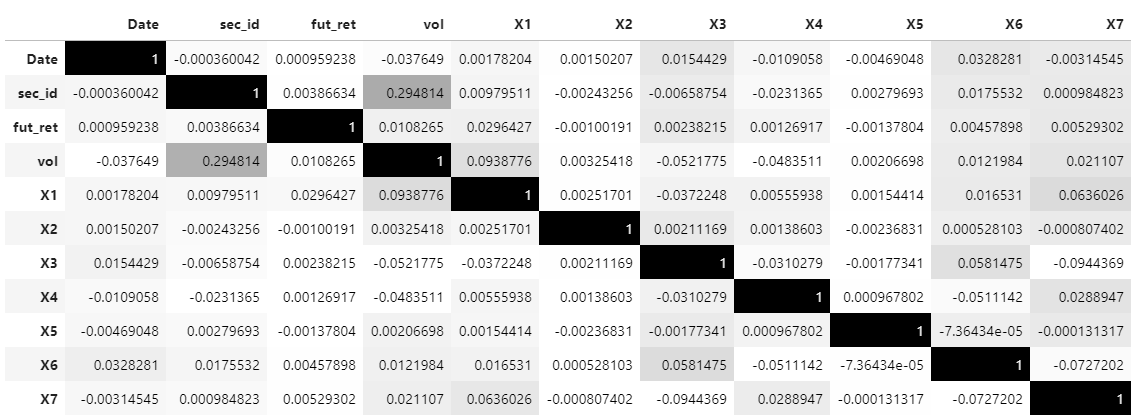
\includegraphics[scale=0.7]{corr_heatmap.PNG}
\caption{pairwise correlation heatmap}
\label{fig:label}
\end{figure}

\noindent Here we find "sec\_id" has a strong positive correlation with volatility. Therefore, we can probably deduce that stocks in our universe are ordered by capitalization size in a decreasing way, since low cap size companies are not liquid enough, and therefore tend to have larger volatilities.\\
\indent This also tells us that label "vol" has relative less noise. We will use this finding later.\\
\indent Now let's have a look at the population histogram on the next page.
\begin{figure}[ht]
\centering
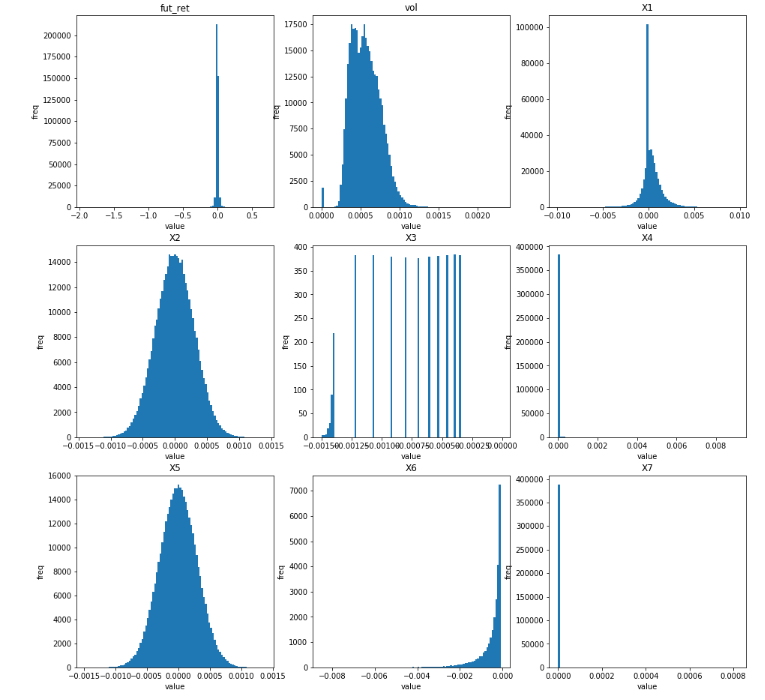
\includegraphics[scale=1]{pop_hist.PNG}
\caption{population histogram for each feature}
\label{fig:label}
\end{figure}

As discussed above, "X2" and "X5" are very likely to be pure white noise (or at least the cases where white noise just overwhelms our signal), because they are bell-shaped, and not skewed. "X1" has a large portion of data close to 0. Therefore, I think though there is some composition of white noise in "X1", it is not pure noise. Let's justify this assumption in the following section.

\subsection{Features Dominated by Random Noise}
\indent One way to further investigate whether a feature "X*" is noise is that for each ticker, we plot the 1st, 2nd and 3rd moment of "X*" across the time, and see if the value varies across each ticker.
\begin{itemize}
    \item If it does not vary, "X*" is probably noise.
    \item Otherwise "X*" may contain some information.
\end{itemize}

\begin{figure}[H]
\centering
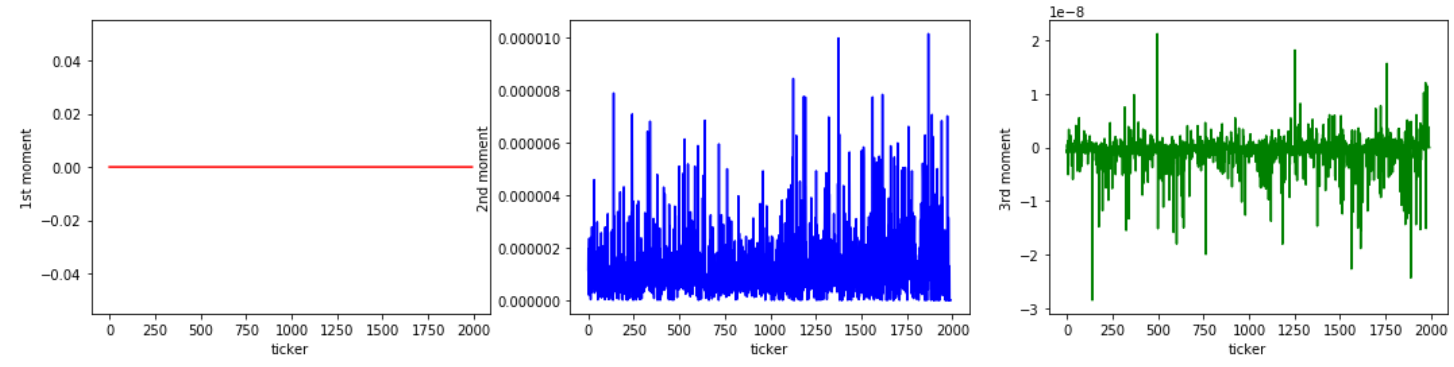
\includegraphics[scale=0.52]{moments_x1.PNG}
\caption{1st, 2nd and 3rd moments of "X1" across different tickers}
\label{fig:label}
\end{figure}

\begin{figure}[H]
\centering
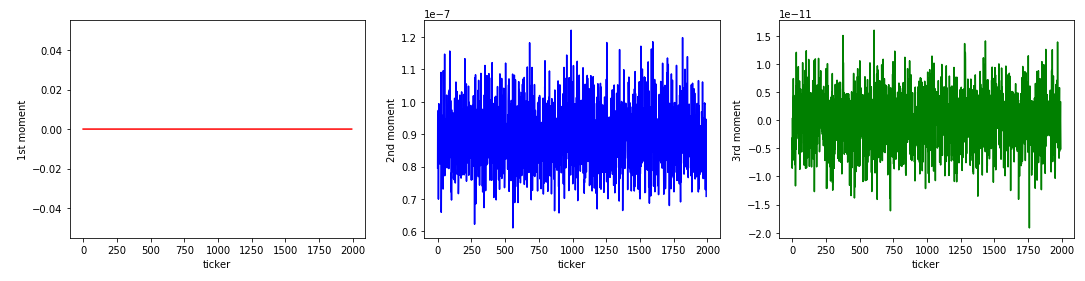
\includegraphics[scale=0.7]{moments_x2.PNG}
\caption{1st, 2nd and 3rd moments of "X2" across different tickers}
\label{fig:label}
\end{figure}

\begin{figure}[H]
\centering
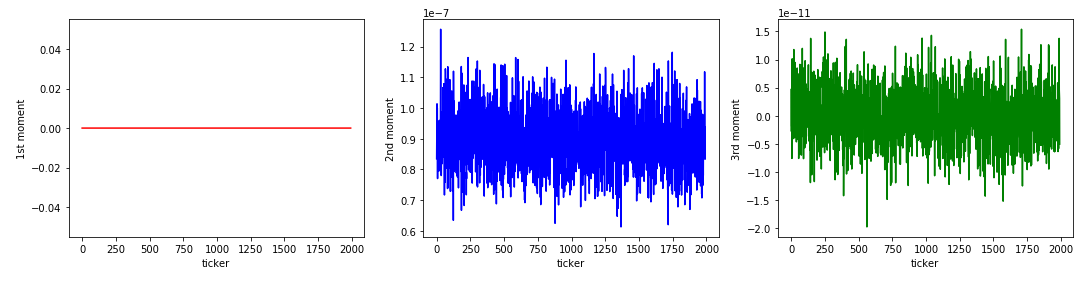
\includegraphics[scale=0.7]{moments_x5.PNG}
\caption{1st, 2nd and 3rd moments of "X5" across different tickers}
\label{fig:label}
\end{figure}

\indent We can find moments of "X1", "X2" and "X5" as above. From the 2nd and 3rd moment, there is some information in "X1", while there is no pattern in moments of "X2" and "X5". We will only drop "X2" and "X5".

\subsection{Deal with Missing Values}
In raw data, all features except for "vol" do not have np.nan, while "vol" has 30,098 np.nans. But after reshaping the data such that each feature as well as return is a dataframe, indexed by date with each ticker per column, we actually find that all features except for "vol" have 5,861 np.nans, while "vol" have $5861+30098=35959$ np.nans. This is probably because that in original raw data, different stocks have slightly different time stamps.\\
\indent After further tests, we find that 1,541 (77.4\% of total) tickers and 12 (6\% of total) dates have np.nan. There is no way we can just drop a whole column or row in our dataframe.\\
\indent Before starting to solve this problem, we first point out that there are two most common possibilities for missing values in a time series:
\begin{itemize}
    \item[1.] A few np.nans lie among valid data in a time series.
    \item[2.] A big chunk of np.nans at the beginning (or in the middle) of our time period.
\end{itemize}

\noindent We can probably use some kind of moving average to fill the np.nans in case 1; but we have to treat case 2 more seriously. Let's deal with np.nans in features except for 'vol' first.

\subsubsection{np.nans in Features other than "vol".}
Due to our discussion above, in different feature dataframes (such as "fut\_ret" and "X7"), all np.nans are in the same place. So if we fill the missing values using some moving average (such as exponential moving average), we will get $\frac{5861}{392539}\approx1.5\%$ of our data points among which all the features are just filled in artificially.\\
\indent Thus we have to drop them in the end and leave the time stamps of different stocks somewhat not identical.

\subsubsection{np.nans in "vol"}
"vol" is a label with relative small noise and lots of np.nans. We have to fill (at least some of) them in some way.\\
\indent One way to fill np.nan is to use exponential moving average. We implement the moving average using historical data in order to avoid lookahead bias. But there is one parameter we have to decide: the center of mass (or effective lag) of our moving average. There are two concerns:
\begin{itemize}
    \item we do not want to use a very long window length, because that will incorporate too much old information;
    \item we do not want to use a rather short window length either, because it will inherit the noise of its previous observations.
\end{itemize}
\noindent Therefore, we have to do some kind of parameter tuning.\\

\indent Notice that "sec\_id" has a strong correlation with "vol". Thus, one way to decide is that we try different window lengths of filling volatility, and pick the one with the strongest correlation with "sec\_id". (Note that we actually think that "sec\_id" is ranked by capitalization size.) 

\begin{figure}[ht]
\centering
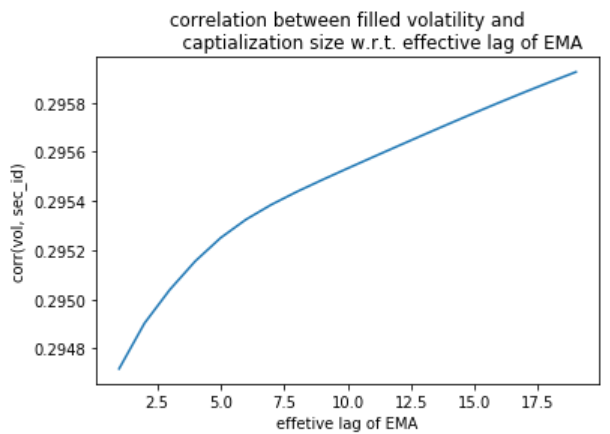
\includegraphics[scale=0.6]{corr_vol_sec_id.PNG}
\caption{correlation with EMA-filled volatility w.r.t. sec\_id}
\label{fig:label}
\end{figure}

\noindent We are disappointed to see that the correlation keeps going up, and a EMA with  $lag>15$ actually does not make sense. Thus, we turn to the second strongest correlation: "vol" and "X1".

\begin{figure}[ht]
\centering
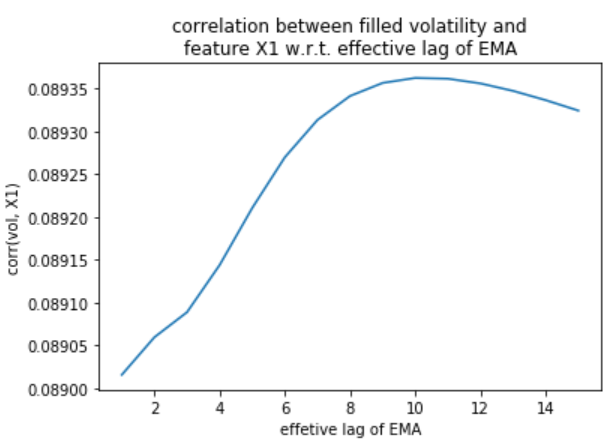
\includegraphics[scale=0.6]{corr_vol_x1.PNG}
\caption{correlation with EMA-filled volatility w.r.t. X1}
\label{fig:label}
\end{figure}

\noindent Based on the plot, we will choose $lag=10$.\\
\indent We also need to test if there are multiple consecutive np.nans in our time series. In order to investigate on this problem, we use exponential moving average to fill "vol" multiple times. If the number of np.nan keeps decreasing, we actually have consecutive np.nans in the middle of our dataframe. The chart is as below.

\begin{figure}[ht]
\centering
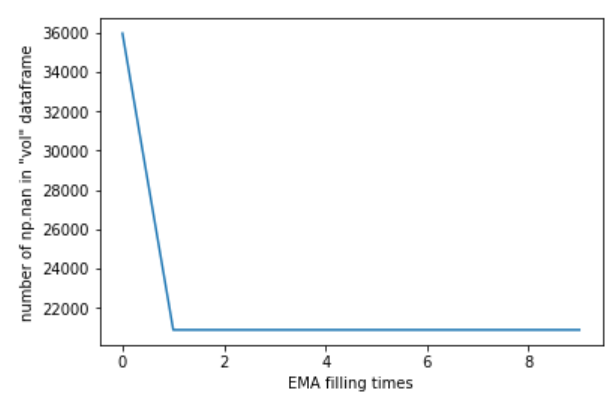
\includegraphics[scale=0.6]{multiple_fill_nan_num.PNG}
\caption{number of np.nans in "vol" w.r.t. filling times using exponential moving average}
\label{fig:label}
\end{figure}

Thus, after filling once, the number of np.nan does not further decrease any more. This indicates that there are no consecutive (i.e., more than one) np.nans in the middle of our "vol" dataframe.

\indent After filling with exponential moving averages, we can find that there are still 20,887 np.nans in "vol". The plot showing the number of np.nan with respect to date can be found as below.
\begin{figure}[ht]
\centering
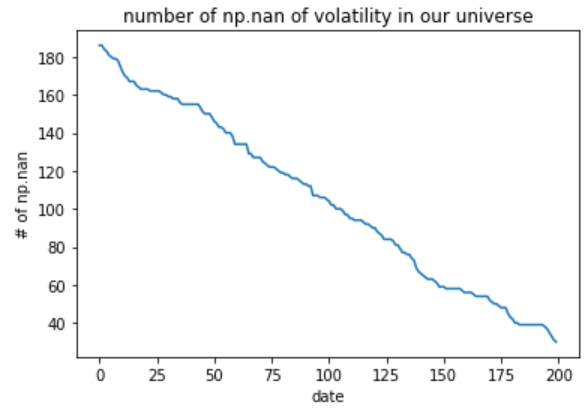
\includegraphics[scale=0.6]{num_of_nan.PNG}
\caption{number of np.nan of volatility w.r.t. date}
\label{fig:label}
\end{figure}

Here we kind of know what is going on. As time goes by, the number of np.nan in volatility dataframe decreases monotonically. It is very likely to be the case that some stocks do not have any observation of volatility at the beginning; but later more and more stocks tend of have valid volatility observations. Thus we will adopt the simplest way: just leave all remaining np.nans unfilled. The intuition behind it is that we have no reason to treat a np.nan the same as 0, because the latter is a valid value, whereas the former is not.

\subsection{Normalize Data}
The final step is to normalize our data. We set our features into four sets and treat them differently:
\begin{itemize}
    \item[1.] sec\_id, Date: we will divide each value by the sample maximum.
    \item[2.] X2, X5: we will not normalize them because we will drop them in the end anyway.
    \item[3.] vol: we will first add a minor positive number ($10^{-4}$) in order to avoid numerical error, and then take log and compute z-score. New feature will be named "log\_vol".
    \item[4.] X1, X3, X4, X6, X7: we will compute z-score of them directly. New features will be named 'X*\_norm'. %among these features, most values are 0. So a more natural way to compute z-score is that we keep the 0s and normalize across other non-zero data.
\end{itemize}
%Note that we want to keep the 0s in case 4 because of that 0 value will be seen as inactive in machine learning models (such as OLS and NN).

\indent In conclusion, in the final data, we have the following columns: Date, sec\_id, fut\_ret, vol, log\_vol, X1, X3, X4, X6, X7, X1\_norm, X3\_norm, X4\_norm, X6\_norm, X7\_norm.

%%%%%%%%%%%%%%%%%%%%%%%%%%%%%%%%%%%%%%%%%%%%%%%%%%%%%%%5
%%%%%%%%%%%%%%%%%%%%%%%%%%%%%%%%%%%%%%%%%%%%%%%%%%%%%%%%5


\section{Regression}
\subsection{Different Regressions}
To start evaluating the predictability of the current data, we start of with OLS to get a general views. We first utilize all data and features for the regression. The out of sample R-square ends up at 11.6 bps. Basically, the result is saying that prediction is barely better than mean.\\
\indent Therefore, we look at the predictions and compare them with the actual data. We see that the actual data is much more scattered than our predictions (See figure: Prediction vs. Actual).

\begin{figure}[H]
\centering
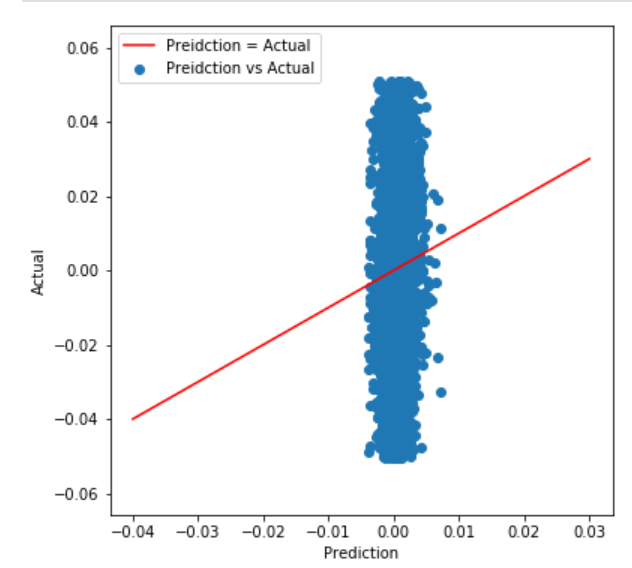
\includegraphics[scale=0.5]{Reg_Pred_vs_Act.PNG}
\caption{Prediction vs. Actual}
\label{fig:label}
\end{figure}

\indent Then We suspect that there may be too many outliers that affect our predictions. We use Median Absolute Deviation (MAD) to clip data with future return greater than (less than) + (-) 4. However, $R^{2}$ decreases.\\
\indent Given our finance intuition, we sometimes notice that when there are multiple signals in the same period, market may react to the strongest signal. So we try to pick the most positive and negative signal among X1, X3, X4, X6, X7 and set the less strong signal to be 0. As the result of this data manipulation, out of sample $R^2$ has no improvement.\\
\indent We also try to have 2 models based on the SEC ID, but the result has a small improvements, almost 12bps.\\
\indent LASSO and Ridge provide similar in sample and out sample $R^{2}$ since we have a large data set and we have already picked out two variables that we believe are random noise. Therefore LASSO and Ridge cannot become very helpful in this case.\\
\indent Interesting, using LASSO enable us to observe the change of variable coefficients. It turns out Date and SEC ID drop to 0 first as penalty increases while X1 stays till the end (See figure: Coefficients of Variables as Penalty Increases).

\begin{figure}[H]
\centering
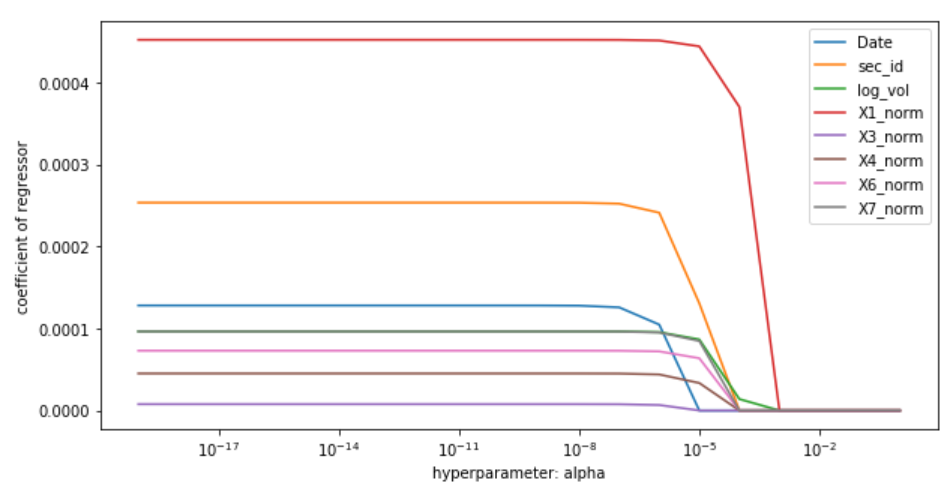
\includegraphics[scale=0.6]{LASSO.PNG}
\caption{Coefficients of Variables as Penalty Increases}
\label{fig:label}
\end{figure}

\indent After experimenting with different regression models, we wonder if something more sophisticated like Light GBM will give us any surprises. However, it turns out Light GBM is only better at fitting in sample data.\\





\subsection{Models Result}
(See figure:$R^{2}$ of Different Models).
\begin{figure}[ht]
\centering
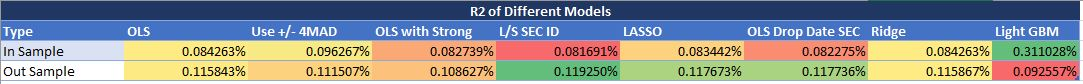
\includegraphics[scale=0.6]{Regression_Performance_V2.JPG}
\caption{$R^{2}$ of Different Models}
\label{fig:label}
\end{figure}


%%%%%%%%%%%%%%%%%%%%%%%%%%%%%%%%%%%%%%%%%%%%%%%%%%%%%%
%%%%%%%%%%%%%%%%%%%%%%%%%%%%%%%%%%%%%%%%%%%%%%%%%%%%%%


\section{Tree and Random Forest}
\subsection{Data}
Since the tree algorithm won't be influenced by order-preserving transformation, so the only important parts is how we deal with default values and outlier. The volatility I used is log-vol, because other teammates may need this, and log has no influence on my model. About feature X1 to X7, we find out that there are a lot of zeros. So we think zeros may mean something different. But I first tried default setting, which is all the features are split by a random chosen number.

\subsection{Default Tree and Forest}
\indent About the parameters in the tree, I use cross validation to get the best. And it turns out that the only important parameter is the depth of the tree. Following is the cross validation plot about the depth.

\begin{figure}[H]
\centering
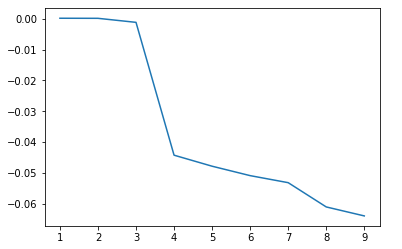
\includegraphics[scale=0.5]{depth_on_default_tree.png}
\caption{cv for default tree}
\label{fig:label}
\end{figure}

\indent We can see that 3 is the best depth for one single tree, which we think is not that reasonable, since we have 7 features in total. But still, we tried to use random forest on this tree to see the result.\\

\indent The next thing we did is to use the cross validation to get the best parameters for forest. Again, the only important parameter here is the total numbers of trees. Figure 14 is a picture of the cross validation and $r^2$ result.

\begin{figure}[htbp]
\centering
\begin{minipage}[t]{0.48\textwidth}
\centering
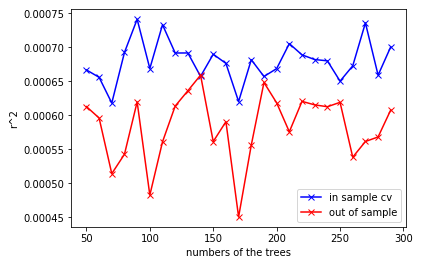
\includegraphics[scale=0.4]{cv_and_r^2_for_forest.png}
\caption{cv for defalut tree}
\end{minipage}
\begin{minipage}[t]{0.48\textwidth}
\centering
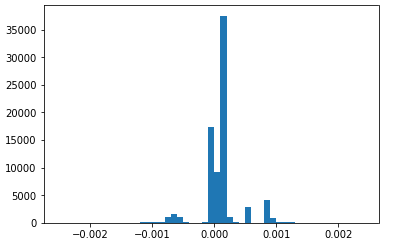
\includegraphics[scale=0.4]{hist_of_default_.png}
\caption{hist of default tree}
\end{minipage}
\end{figure}


\indent Actually on average, 100 to 300 hundreds trees give us a similar result.The out-of-sample $r^2$ for this model is about 6 bps. Following is the hist of the out-of-sample output.\\
\indent From Figure 15, we can see that this predictor is just predicting the mean values. And also, there is no obvious tail effect in this distribution, which is disobey our opinion on future return.

\subsection{Self-designed Tree and Forest}
\indent We think this model has a problem which is the it randomly split feature X1 to X7. By observation, we find that there are a lot of zeros in those features, so we think 0 should mean something different from non-zero values. So we change the tree like this: if a feature has a lot of 0, we first see whether 0 is a good split point. If it is, we use 0 to split. After this, we randomly choose values from non-zero values to split the points.\\
\indent Again we do the cross validation for both single tree and forest. Following is the cross validation result for one single tree.

\begin{figure}[htbp]
\centering
\begin{minipage}[t]{0.48\textwidth}
\centering
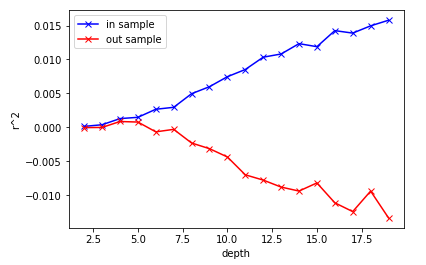
\includegraphics[scale=0.4]{cv_for_our_tree.png}
\caption{cv of self-designed tree}
\end{minipage}
\begin{minipage}[t]{0.48\textwidth}
\centering
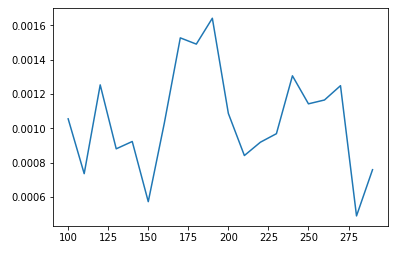
\includegraphics[scale=0.4]{cv_our_forest.png}
\caption{cv of self-designed forest}
\end{minipage}
\end{figure}

\indent From Figure 16, we can see that the best depth now is 6 or 7, so we finally choose 7 as the best depth and build the forest. Following is the cross validation on the forest.\\
\indent From Figure 17, we can see that 170 to 190 gives me a similar result, so we finally choose 190 as the best parameter. Following is the hist for the out-of-sample output.

\begin{figure}[htbp]
\centering
\begin{minipage}[t]{0.48\textwidth}
\centering
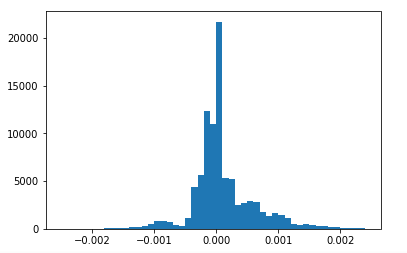
\includegraphics[scale=0.4]{hist_our_forest.png}
\caption{hist of self-designed forest}
\end{minipage}
\begin{minipage}[t]{0.48\textwidth}
\centering
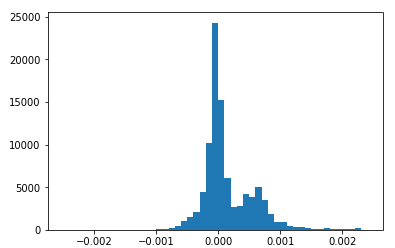
\includegraphics[scale=0.4]{hist_for_random.png}
\caption{hist of new forest}
\end{minipage}
\end{figure}

\indent From Figure 18, now we can see that the there is a fat tail on the distribution, which is in accordance with our common sense. Also, the average out of sample $r^2$ is about 12-13 bps.\\

\subsection{Adding More Randomness}
\indent The last thing we did is that we want to add more randomness in this model, so we change the tree as following, on each node, we randomly select 1/3 features, and use the best from them. Following is the hist for this model.\\
\indent The correlation of this model is about $60\% $ compared to the former one, and the out of sample $r^2$ is about 10-11 bps. From Figure 19, we can still see a fat tail in this distribution, so we finally use both of these models to do the aggregation.\\

%%%%%%%%%%%%%%%%%%%%%%%%%%%%%%%%%%%%%%%%%%55
%%%%%%%%%%%%%%%%%%%%%%%%%%%%%%%%%%%%%%%%%


\section{Neural Network}
\subsection{Data}
The version of data used in Neural Network is v3. Firstly we dropped all row with NAN vol. Then we replaced 0 vol with the minimum value of vol column. Doing this, we assume the 0 vol caused by very low liquidity within observing window, rather than missing value.

After get rid of all zero and missing vol in data, we generated a new column of fut\_ret/vol. In Neural Network models, instead of predicting fut\_vol, we predict fut\_ret/vol. Before calculating R-square, we multiply our prediction by vol to get our prediction for fut\_vol.

In this section, the package we used is \textit{torch}. We split data into 2:2:6 portion and use them as test, validation and training data. Due to the limitation of computation ability, we did not use cross validation to tune the hyper parameter and only tuned them on a grid. 

\subsection{Module}
In order to build a fine tuned network for this problem, we tried different module.
\begin{itemize}
    \item Activation: We tried PReLU and it is better than vanilla ReLU
    \item Drop Layer: We add $p=0.5$ drop layer after each fully connected layer, when the number of neurons is big. 
    \item Regularization: we add L1/L2 regularization term in our optimizer to shrink the weights.
    \item Batch Normalization: We normalize the output of each hidden layer.
\end{itemize}


\subsection{Observation and Best Network}
\subsubsection{Observation}
We observed that after build the neural network deep, it tends to predict the mean value of whole set's fut\_ret. This will lead to very low even negative R square. No matter how we change hyper parameters, after the network converges, this phenomenon happens.

\begin{figure}[ht]
    \centering
    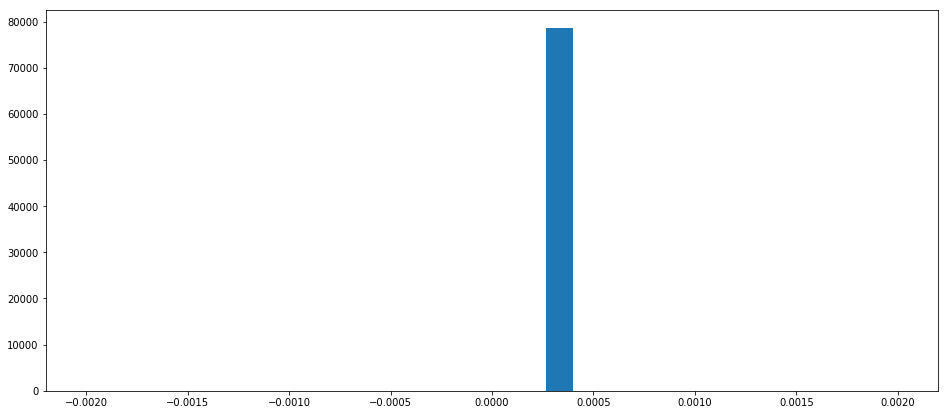
\includegraphics[scale=0.22]{NN_2.png}
    \caption{Deep NN's Prediction}
    \label{fig:label}
\end{figure}

To avoid this, we can only apply very simple network structure. We did not benefit from depth of neural network.


\subsubsection{Best Result}
The best tuned hyper-parameters are given below.
\begin{itemize}
    \item one hidden layer, four neurons
    \item no drop layer
    \item with batch normalization
    \item with l2 regularization, alpha 1e-1
    \item use PReLU as activation function
    \item use Adam as optimizer, learning rate 1
\end{itemize}

This network gives 5-9 bps in-sample R square and 7-12 bps out-of-sample R square. The variation mainly due to randomness in initialization. Here we use HE normal initialization.

Here we draw histogram of our prediction. In Figure 21, the left is our prediction's histogram and the right is real fut\_ret histogram. This two pictures are in same scale. We can see our prediction is near 0. Though it cannot capture the fat tail of return. It can mainly predict rise or drop.

If we zoom in, we can see our prediction's histogram more clearly from Figure 22.

\begin{figure}[htbp]
\centering
\begin{minipage}[t]{0.48\textwidth}
\centering
\includegraphics[width=7cm]{nn_2.png}
\caption{histogram of prediction}
\end{minipage}
\begin{minipage}[t]{0.48\textwidth}
\centering
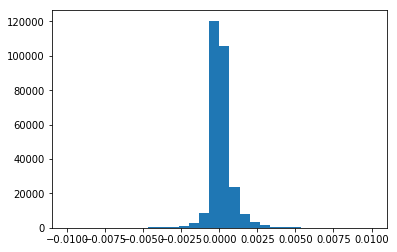
\includegraphics[width=5cm]{nn_3.png}
\caption{histogram of prediction, zoom in}
\end{minipage}
\end{figure}

%%%%%%%%%%%%%%%%%%%%%%%%%%%%%%%%%%%%%%%%%%%%%%%%%55
%%%%%%%%%%%%%%%%%%%%%%%%%%%%%%%%%%%%%%%%%%%%%%%%%%%%5

\section{Aggregation}
In this section, we want to aggregate all our existing models with decent performance. We have six models, and they are Neural Network, Light GBM, two Regression models with different selected features, two Random Forest one of which add more randomness. You can find detail of all these models from previous sections. They all have near 10 bps R square in test case.

\subsection{Methodology}
In sense of aggregation, we want to build two layers model. As for lower layer, it refers to six decent models we already build in previous sections. We want to use the prediction of these 6 models as input columns for upper level model. So for upper layer, it uses prediction of different lower level models and predict the fut\_ret. 

We train six fine tuned existing models on first 150 days, and gives out-of-sample prediction for latter 50 days. Then we split latter 50 days into training and test set for upper layer model. The first three quarter of latter 50 days is training set for upper layer model, and last quarter is test set.

From this point, when we mention train or test, we refer to upper layer model. So both train and test are from latter 50 days of our data.


\subsection{How to Deal with NaN}
In vol column, there is lots of NaN. There are two ways to deal with this problem. First way is, we fill all NaN value with 0, which is a consistent way. And second way is, we assume the data with NaN vol has different property from data with non-NaN vol, and model them differently.

For these two methods, the lower level models have similar performance. But after aggregation, the upper level give different results. It turns out, the second way gives us higher R square. So from this point, we adopt second way.

As for how to model data with NaN vol, we use linear regression on X1 to X7. Because we have an observation that when vol is NaN, 99\% of data gives 0 fut\_ret. Instead of giving 0 prediction, which is a kind of data-driven, we use linear regression, the most explainable model to predict.

So when we do the test, firstly we split the data to two according to whether vol is NaN or not. Than we use two-layer model to predict non-NaN vol data, and linear regression to predict NaN vol data. Then we join these predictions together as our final result.


\subsection{Method}
First, we see the correlation of predictions on training set from lower level models. Note that, training set is in sense of upper level model,it is still test set for lower level models.


\begin{figure}[ht]
    \centering
    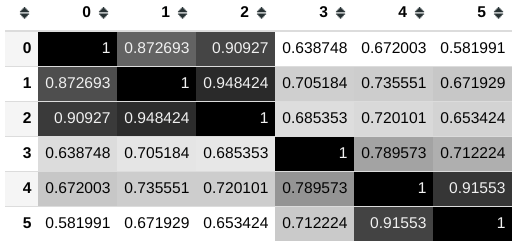
\includegraphics[scale=0.8]{agg_1.png}
    \caption{Correlations between features in training set}
    \label{fig:label}
\end{figure}

Now we build model for upper level. The methods we tried list in below.
\begin{itemize}
    \item Neutral Network: Even after the simplest net, the prediction is mean of data, which is the same problem we talked in previous section.
    \item OLS: Bad approach, as there is high correlation between features
    \item Lasso: very small penalty(1e-7) leads to choose only one feature. We let it choose two features, otherwise upper level do not add value.
    \item Ridge
    \item Random Forest
    \item Light GBM
\end{itemize}
Figure 24 gives all train and test R square from lower level models and upper level models we tried. \pagebreak

\begin{figure}[ht]
    \centering
    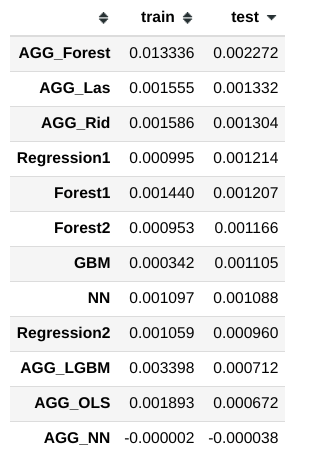
\includegraphics[scale=0.5]{agg_2.png}
    \caption{Results(in order of test R square)}
    \label{fig:label}
\end{figure}

So aggregating did give us better result. We choose Random Forest aggregation with 6 other models as our final choice.

When using random forest as our upper level model, feature importance is:
    \begin{itemize}
        \item Neural Network: 0.26931832
        \item Regression 1: 0.1825856
        \item Random Forest 1: 0.17319282
        \item Random Forest 2:0.14946527
        \item Regression 2: 0.13878568
        \item Light GBM: 0.08665231
    \end{itemize}








%%%%%%%%%%%%%%%%%%%%%%%%%%%%%%%%%%%%%%%%%%%%%%%%%%%%%%
%%%%%%%%%%%%%%%%%%%%%%%%%%%%%%%%%%%%%%%%%%%%%%%%%%%%%%
\section{Further Possible Improvements}
After the final presentation, we actually find that there may still be some possible improvements to further enhance our prediction. One (and probably the most important one) is to use "fut\_ret"/"vol" rather than "vol" itself as the dependent variable and exclude "vol" from our regressors.

\end{document}
